

\section{Self Force}

A test particle orbiting a blackhole follows a geodesic, which is the path of extremal proper time. This is described by the geodesic equation,
\begin{equation}
\frac{d^2x^\mu}{d\tau^2}+\Gamma^\mu_{\rho\sigma}\frac{dx^\rho}{d\tau}\frac{dx^\sigma}{d\tau}=0
\end{equation}
where $\tau$ is the proper time and $\Gamma^\mu_{\rho\sigma}$ is the Christoffel symbol, given by~\cite{Carroll}
\begin{equation}
\Gamma^\sigma_{\mu\nu}=\frac{1}{2}g^{\sigma\rho}(\partial_\mu g_{\nu\rho}+\partial_\nu g_{\rho\mu} - \partial_\rho g_{\mu\nu})
\end{equation}

However, a blackhole, of any size, is not a test particle. In the limit of an EMRI, the additional force can be treated perturbatively in the mass ratio of the two particles, in the relativistic case. In the scalar case, the self force is simply written as a delta function source to the wave equation dependent upon the particle's position in time~\cite{WardellSelfForceReview}
\begin{eqnarray}
  \Box\Psi^{ret}=-4\pi q\int\delta_4(x,z(\tau^\prime))d\tau^\prime
\end{eqnarray}
In this equation, $\Box$ is the D'Alembertian and $z(\tau^\prime)$ is the evolving path of the source in spacetime as a function of the particle's proper time. The retarded field $\Psi^{ret}$, is defined to be the field determined by physics taking place at $t_r=t-\frac{|\vec{r}-\vec{r}^\prime|}{c}$; that is, at some distance away from the particle's path, the physical effects of gravity on the scalar field are retarded by light travel time. In the scalar approximation, the particle acts as a delta function point source, with a charge of $q$ and mass $m$. That charge may accelerate or evolve with time; see chapter~\ref{futurework}. 

The retarded field is singular at the location of the particle due to the delta function source. Singularities are computationally problematic. To regularize this singularity, a regular field is created through the use of an effective source.
\begin{eqnarray}
\Psi^R=\Psi^{ret}-\Psi^S\\
\Box\Psi^R=S_{eff}\\
S_{eff}=q\delta(x,x_0)-\Box(W\Psi^S)\\
F_\alpha=(\nabla_\alpha\Psi^r)|_{x=x_0}
\end{eqnarray}
The regularized field, $\Psi^R$, is defined in terms of the retarded field with the singular field, $\Psi^S$, subtracted. This leads to the definition of an effective source, $S_{eff}$, that is zero inside the neighborhood of the particle, due to the world tube window function around the particle, shown in Figure~\ref{wtwindow}, and that approximates the source outside that region. Outside that region, the regularized field is equal to the retarded field. The self-force can be derived from the final equation given above, $F_\alpha$ is merely a gradient of the field itself~\cite{vega_wardell_diener_eff_source}. 


\subsection{World tube}
\begin{figure}
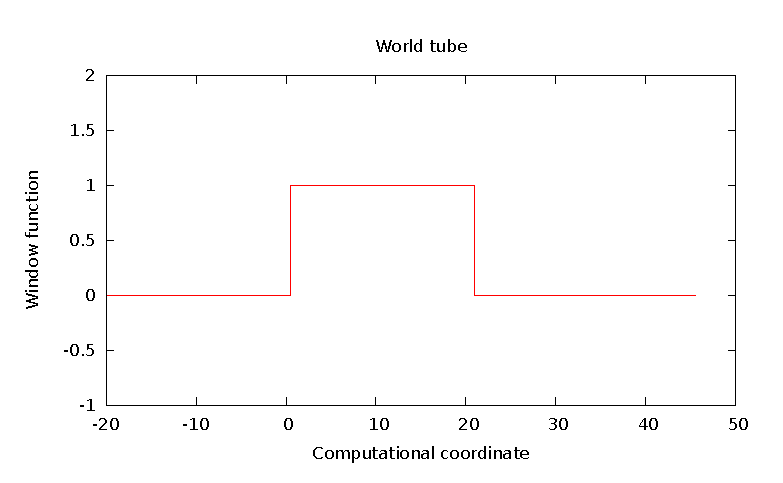
\includegraphics{worldTubeItself}
\caption{Spatial slice of the world tube window function.}
\label{wtwindow}
\end{figure}

The world tube window function around the particle carves out a ring around the blackhole in the orbital plane, due to the use of spherical harmonics to increase the dimensionality of space. In my C++ code, the world tube extends throughout the entire tortoise region, ending at the transitions to the hyperboloidal regions. When calculating numerical fluxes at this boundary, it is necessary to account for both the coordinate transformations between either side of the boundary and the transformation between regular and retarded field.

While on a circular orbit, the particle follows a fixed path that prevents it from inspiraling. This does not conserve energy, since energy is radiated away into the blackhole and to infinity by the scalar waves. Clearly, we are artificially inputting energy into the simulation by holding the particle fixed on its orbit. This, in a nutshell, explains the need for scalar (or gravitational) radiation, and for self force in this limit. 


\section{Comparison between C++ and Fortran codes}

I've performed extensive comparisons between Peter Diener's Fortran code~\ref{heffernan_ottewil_wardell_modesum_basisForCode}, implementing the same thing, and my C++ code. To roundoff precision, they agree, as evidenced by the near-machine-precision ($10^{-15}$) levels of agreement in both absolute and relative error that I achieve in Figures~\ref{circ1},~\ref{circ2},~\ref{circ3}, and~\ref{circ4}

\begin{figure}
  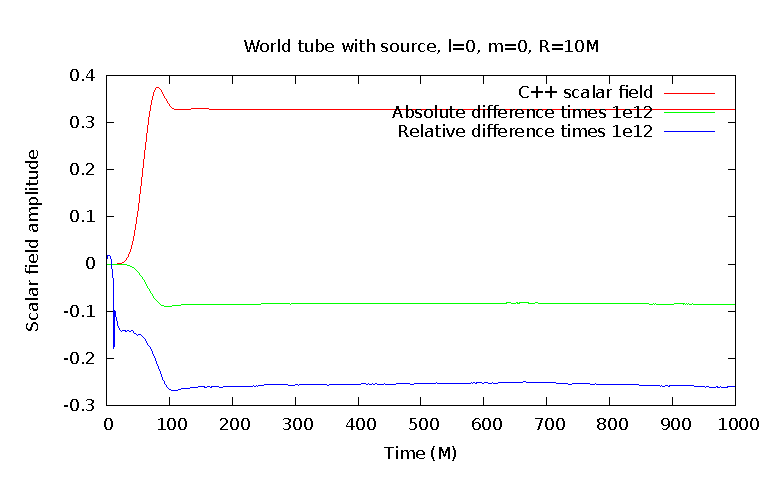
\includegraphics{wtcircl0m0}
  \caption{Comparison between Fortran and C++ codes for a particle on a circular orbit, l=0, m=0.}
  \label{circ1}
\end{figure}
\begin{figure}
  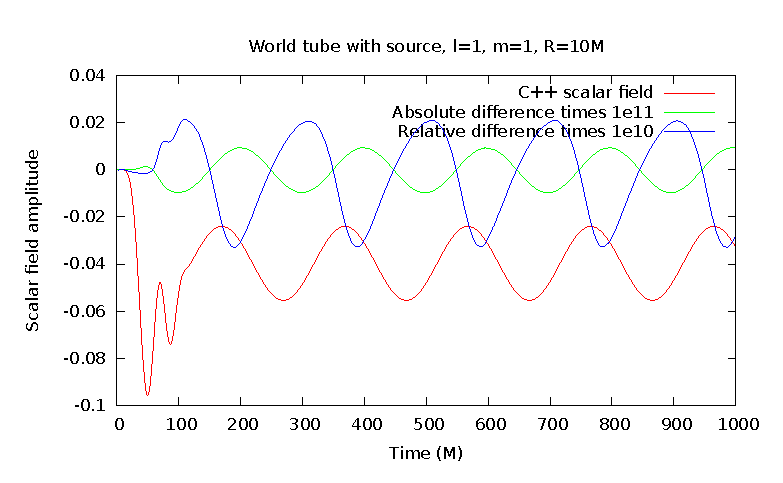
\includegraphics{wtcircl1m1}
  \caption{Comparison between Fortran and C++ codes for a particle on a circular orbit, l=1, m=1.}
  \label{circ2}
\end{figure}
\begin{figure}
  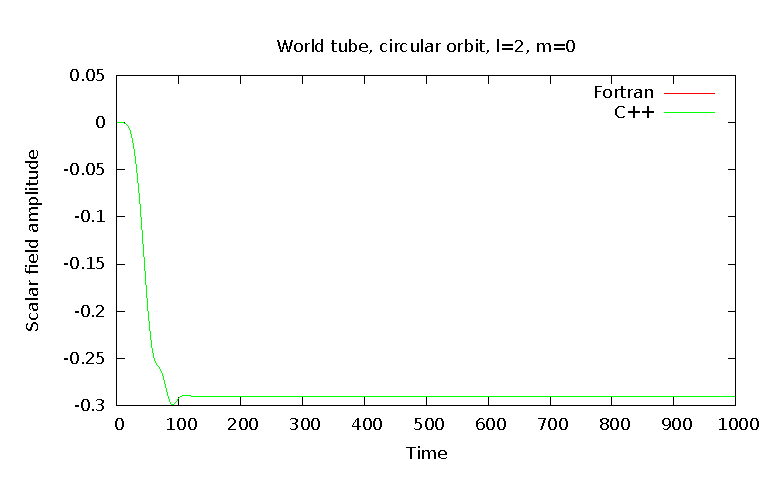
\includegraphics{wtcircl2m0}
  \caption{Comparison between Fortran and C++ codes for a particle on a circular orbit, l=2, m=0.}
  \label{circ3}
\end{figure}
\begin{figure}
  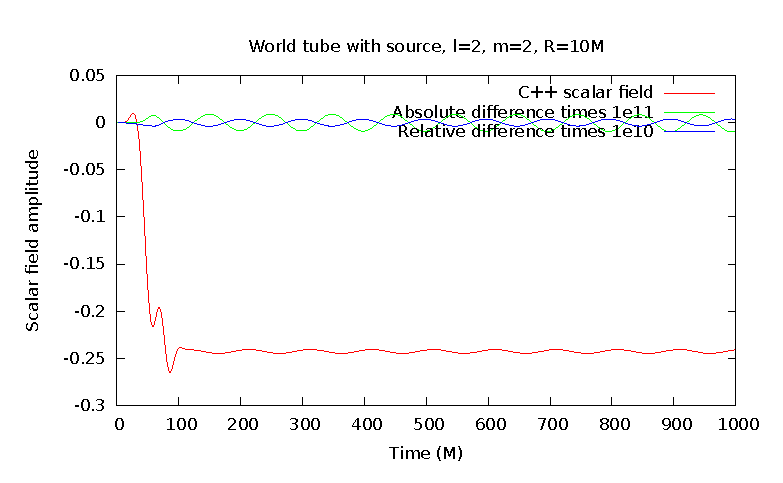
\includegraphics{wtcircl2m2}
  \caption{Comparison between Fortran and C++ codes for a particle on a circular orbit, l=2, m=2.}
  \label{circ4}
\end{figure}
